%\SweaveUTF8
\documentclass[aspectratio=169]{beamer}

\usetheme{default}
% Slide setup, colour independent

\usepackage{amsmath,amssymb,amsthm}
\usepackage[utf8]{inputenc}
\usepackage{colortbl}
\usepackage{bm}
\usepackage{xcolor}
\usepackage{dsfont}
\usepackage{setspace}
%\usepackage{subfigure}
% To use \ding{234} and the like
\usepackage{pifont}
% To cross reference between slide files
\usepackage{zref-xr,zref-user}
% Use something like
% \zexternaldocument{fileI}
% in the tex files. And cite using \zref instead of \ref
\usepackage{booktabs}
\usepackage{marvosym}
\usepackage{cancel}
%\usepackage{transparent}

% Fields and the like
\def\IC{\mathbb{C}}
\def\IE{\mathbb{E}}
\def\IF{\mathbb{F}}
\def\II{\mathbb{I}}
\def\IJ{\mathbb{J}}
\def\IK{\mathbb{K}}
\def\IM{\mathbb{M}}
\def\IN{\mathbb{N}}
\def\IP{\mathbb{P}}
\def\IR{\mathbb{R}}
\def\IZ{\mathbb{Z}}
\def\11{\mathds{1}}


% Bold lowercase
\def\ba{\bm{a}}
\def\bb{\bm{b}}
\def\bc{\bm{c}}
\def\bd{\bm{d}}
\def\be{\bm{e}}
\def\bf{\bm{f}}
\def\bh{\bm{h}}
\def\bi{\bm{i}}
\def\bj{\bm{j}}
\def\bk{\bm{k}}
\def\bn{\bm{n}}
\def\bp{\bm{p}}
\def\br{\bm{r}}
\def\bs{\bm{s}}
\def\bu{\bm{u}}
\def\bv{\bm{v}}
\def\bw{\bm{w}}
\def\bx{\bm{x}}
\def\by{\bm{y}}
\def\bz{\bm{z}}

% Bold capitals
\def\bB{\bm{B}}
\def\bD{\bm{D}}
\def\bE{\bm{E}}
\def\bF{\bm{F}}
\def\bG{\bm{G}}
\def\bI{\bm{I}}
\def\bL{\bm{L}}
\def\bN{\bm{N}}
\def\bP{\bm{P}}
\def\bR{\bm{R}}
\def\bS{\bm{S}}
\def\bT{\bm{T}}
\def\bX{\bm{X}}

% Bold numbers
\def\b0{\bm{0}}

% Bold greek
\bmdefine{\bmu}{\bm{\mu}}
\def\bphi{\bm{\phi}}
\def\bvarphi{\bm{\varphi}}
\def\bPi{\bm{\Pi}}
\def\bGamma{\bm{\Gamma}}

% Bold red sentence
\def\boldred#1{{\color{red}\textbf{#1}}}
\def\defword#1{{\color{orange}\textbf{#1}}}

% Caligraphic letters
\def\A{\mathcal{A}}
\def\B{\mathcal{B}}
\def\C{\mathcal{C}}
\def\D{\mathcal{D}}
\def\E{\mathcal{E}}
\def\F{\mathcal{F}}
\def\G{\mathcal{G}}
\def\H{\mathcal{H}}
\def\I{\mathcal{I}}
\def\L{\mathcal{L}}
\def\M{\mathcal{M}}
\def\N{\mathcal{N}}
\def\P{\mathcal{P}}
\def\R{\mathcal{R}}
\def\S{\mathcal{S}}
\def\T{\mathcal{T}}
\def\U{\mathcal{U}}
\def\V{\mathcal{V}}

% Adding space for prime (') where needed
\def\pprime{\,'}
% Adding space for star (\star) where needed
\def\pstar{{\,\star}}

% tt font for code
\def\code#1{{\tt #1}}

% i.e., e.g.
\def\eg{\emph{e.g.}}
\def\ie{\emph{i.e.}}


% Operators and special symbols
\def\nbOne{{\mathchoice {\rm 1\mskip-4mu l} {\rm 1\mskip-4mu l}
{\rm 1\mskip-4.5mu l} {\rm 1\mskip-5mu l}}}
\def\cov{\ensuremath{\mathsf{cov}}}
\def\Var{\ensuremath{\mathsf{Var}\ }}
\def\Im{\textrm{Im}\;}
\def\Re{\textrm{Re}\;}
\def\det{\ensuremath{\mathsf{det}}}
\def\diag{\ensuremath{\mathsf{diag}}}
\def\nullspace{\ensuremath{\mathsf{null}}}
\def\nullity{\ensuremath{\mathsf{nullity}}}
\def\rank{\ensuremath{\mathsf{rank}}}
\def\range{\ensuremath{\mathsf{range}}}
\def\sgn{\ensuremath{\mathsf{sgn}}}
\def\Span{\ensuremath{\mathsf{span}}}
\def\tr{\ensuremath{\mathsf{tr}}}
\def\imply{$\Rightarrow$}
\def\restrictTo#1#2{\left.#1\right|_{#2}}
\newcommand{\parallelsum}{\mathbin{\!/\mkern-5mu/\!}}
\def\dsum{\mathop{\displaystyle \sum }}%
\def\dind#1#2{_{\substack{#1\\ #2}}}

\DeclareMathOperator{\GL}{GL}
\DeclareMathOperator{\Rel}{Re}
\def\Nt#1{\left|\!\left|\!\left|#1\right|\!\right|\!\right|}
\newcommand{\tripbar}{|\! |\! |}



% The beamer bullet (in base colour)
\def\bbullet{\leavevmode\usebeamertemplate{itemize item}\ }

% Theorems and the like
\newtheorem{proposition}[theorem]{Proposition}
\newtheorem{property}[theorem]{Property}
\newtheorem{importantproperty}[theorem]{Property}
\newtheorem{importanttheorem}[theorem]{Theorem}
%\newtheorem{lemma}[theorem]{Lemma}
%\newtheorem{corollary}[theorem]{Corollary}
\newtheorem{remark}[theorem]{Remark}
\setbeamertemplate{theorems}[numbered]
%\setbeamertemplate{theorems}[ams style]

%
%\usecolortheme{orchid}
%\usecolortheme{orchid}

\def\red{\color[rgb]{1,0,0}}
\def\blue{\color[rgb]{0,0,1}}
\def\green{\color[rgb]{0,1,0}}


% Get rid of navigation stuff
\setbeamertemplate{navigation symbols}{}

% Set footline/header line
\setbeamertemplate{footline}
{%
\quad p. \insertpagenumber \quad--\quad \insertsection\vskip2pt
}
% \setbeamertemplate{headline}
% {%
% \quad\insertsection\hfill p. \insertpagenumber\quad\mbox{}\vskip2pt
% }


\makeatletter
\newlength\beamerleftmargin
\setlength\beamerleftmargin{\Gm@lmargin}
\makeatother

% Colours for special pages
\def\extraContent{yellow!20}


%%%%%%%%%%%%%%%%%
\usepackage{tikz}
\usetikzlibrary{shapes,arrows}
\usetikzlibrary{positioning}
\usetikzlibrary{shapes.symbols,shapes.callouts,patterns}
\usetikzlibrary{calc,fit}
\usetikzlibrary{backgrounds}
\usetikzlibrary{decorations.pathmorphing,fit,petri}
\usetikzlibrary{automata}
\usetikzlibrary{fadings}
\usetikzlibrary{patterns,hobby}
\usetikzlibrary{backgrounds,fit,petri}
\usetikzlibrary{tikzmark}

\usepackage{pgfplots}
\pgfplotsset{compat=1.6}
\pgfplotsset{ticks=none}

\usetikzlibrary{decorations.markings}
\usetikzlibrary{arrows.meta}
\tikzset{>=stealth}

% For tikz
\tikzstyle{cloud} = [draw, ellipse,fill=red!20, node distance=0.87cm,
minimum height=2em]
\tikzstyle{line} = [draw, -latex']


%%% For max frame images
\newenvironment{changemargin}[2]{%
\begin{list}{}{%
\setlength{\topsep}{0pt}%
\setlength{\leftmargin}{#1}%
\setlength{\rightmargin}{#2}%
\setlength{\listparindent}{\parindent}%
\setlength{\itemindent}{\parindent}%
\setlength{\parsep}{\parskip}%
}%
\item[]}{\end{list}}


% Make one image take up the entire slide content area in beamer,.:
% centered/centred full-screen image, with title:
% This uses the whole screen except for the 1cm border around it
% all. 128x96mm
\newcommand{\titledFrameImage}[2]{
\begin{frame}{#1}
%\begin{changemargin}{-1cm}{-1cm}
\begin{center}
\includegraphics[width=108mm,height=\textheight,keepaspectratio]{#2}
\end{center}
%\end{changemargin}
\end{frame}
}

% Make one image take up the entire slide content area in beamer.:
% centered/centred full-screen image, no title:
% This uses the whole screen except for the 1cm border around it
% all. 128x96mm
\newcommand{\plainFrameImage}[1]{
\begin{frame}[plain]
%\begin{changemargin}{-1cm}{-1cm}
\begin{center}
\includegraphics[width=108mm,height=76mm,keepaspectratio]{#1}
\end{center}
%\end{changemargin}
\end{frame}
}

% Make one image take up the entire slide area, including borders, in beamer.:
% centered/centred full-screen image, no title:
% This uses the entire whole screen
\newcommand{\maxFrameImage}[1]{
\begin{frame}[plain]
\begin{changemargin}{-1cm}{-1cm}
\begin{center}
\includegraphics[width=\paperwidth,height=\paperheight,keepaspectratio]
{#1}
\end{center}
\end{changemargin}
\end{frame}
}

% This uses the entire whole screen (to include in frame)
\newcommand{\maxFrameImageNoFrame}[1]{
\begin{changemargin}{-1cm}{-1cm}
\begin{center}
\includegraphics[width=\paperwidth,height=0.99\paperheight,keepaspectratio]
{#1}
\end{center}
\end{changemargin}
}

% Make one image take up the entire slide area, including borders, in beamer.:
% centered/centred full-screen image, no title:
% This uses the entire whole screen
\newcommand{\maxFrameImageColor}[2]{
\begin{frame}[plain]
\setbeamercolor{normal text}{bg=#2!20}
\begin{changemargin}{-1cm}{-1cm}
\begin{center}
\includegraphics[width=\paperwidth,height=\paperheight,keepaspectratio]
{#1}
\end{center}
\end{changemargin}
\end{frame}
}


\usepackage{tikz}
\usetikzlibrary{patterns,hobby}
\usepackage{pgfplots}
\pgfplotsset{compat=1.6}
\pgfplotsset{ticks=none}

\usetikzlibrary{backgrounds}
\usetikzlibrary{decorations.markings}
\usetikzlibrary{arrows.meta}
\tikzset{>=stealth}

\tikzset{
  clockwise arrows/.style={
    postaction={
      decorate,
      decoration={
        markings,
        mark=between positions 0.1 and 0.9 step 40pt with {\arrow{>}},
   }}}}


% Beginning of a section
\newcommand{\newSectionSlide}[1]{
\begin{frame}[noframenumbering,plain]
  \begin{tikzpicture}[remember picture,overlay]
    \node[above right,inner sep=0pt,opacity=0.2] at (current page.south west)
    {
        \includegraphics[height=\paperheight,width=\paperwidth]{#1}
    };
  \end{tikzpicture}
  \setbeamercolor{section in toc}{fg=subsub_header_section}
  \setbeamerfont{section in toc}{size=\Large,series=\bfseries}
  \setbeamertemplate{section in toc shaded}[default][60]
  %\setbeamercolor{background canvas}{bg=section_colour}
  \tableofcontents[
    currentsection,
    sectionstyle=show/shaded,
    subsectionstyle=show/hide/hide,
    subsubsectionstyle=hide/hide/hide]
\end{frame}
\addtocounter{page}{-1}
}

% Beginning of a subsection
\newcommand{\newSubSectionSlide}[1]{
\begin{frame}[noframenumbering,plain]
  \begin{tikzpicture}[remember picture,overlay]
    \node[above right,inner sep=0pt,opacity=0.2] at (current page.south west)
    {
        \includegraphics[height=\paperheight,width=\paperwidth]{#1}
    };
  \end{tikzpicture}
  \setbeamercolor{section in toc}{fg=subsub_header_section}
  \setbeamerfont{section in toc}{size=\Large,series=\bfseries}
  \setbeamertemplate{section in toc shaded}[default][60]
  %\setbeamercolor{background canvas}{bg=section_colour}
  \tableofcontents[
    currentsection,
    sectionstyle=show/hide,
    subsectionstyle=show/shaded/hide,
    subsubsectionstyle=hide/hide/hide]
\end{frame}
\addtocounter{page}{-1}
}



   %%%%%%%%%%%
% To have links to parts in the outline
\makeatletter
\AtBeginPart{%
  \addtocontents{toc}{\protect\beamer@partintoc{\the\c@part}{\beamer@partnameshort}{\the\c@page}}%
}
%% number, shortname, page.
\providecommand\beamer@partintoc[3]{%
  \ifnum\c@tocdepth=-1\relax
    % requesting onlyparts.
    \makebox[6em]{Part #1:} \textcolor{green!30!blue}{\hyperlink{#2}{#2}}
    \par
  \fi
}
\define@key{beamertoc}{onlyparts}[]{%
  \c@tocdepth=-1\relax
}
\makeatother%

\newcommand{\nameofthepart}{}
\newcommand{\nupart}[1]%
    {   \part{#1}%
        \renewcommand{\nameofthepart}{#1}%
        {
          \setbeamercolor{background canvas}{bg=orange!50}
          \begin{frame}{#1}%\partpage 
          \hypertarget{\nameofthepart}{}\tableofcontents%
          \end{frame}
        }
    }


% The title page with figure
\newcommand{\titlepagewithfigure}[1]{%
\begin{frame}[noframenumbering,plain]
  \begin{tikzpicture}[remember picture,overlay]
    \node[above right,inner sep=0pt,opacity=0.2] at (current page.south west)
    {
        \includegraphics[height=\paperheight,width=\paperwidth]{#1}
    };
    \node[anchor=north east,
    inner sep=5pt,
    opacity=0.9] at (current page.north east)
    {
        
\includegraphics[width=0.2\textwidth]{FIGS/UM-logo-horizontal-CMYK.png}
    };
    \node[anchor=south, 
    align=justify, 
    text=black, 
    text width=1.1\textwidth,
    font=\footnotesize]  (land_acknowledgement)
    at (current page.south) 
    {The University of Manitoba campuses are located on original lands of Anishinaabeg, Ininew, Anisininew, Dakota and Dene peoples, and on the National Homeland of the Red River Métis.\\
    We respect the Treaties that were made on these territories, we acknowledge the harms and mistakes of the past, and we dedicate ourselves to move forward in partnership with Indigenous communities in a spirit of Reconciliation and collaboration.};  
    \node[align=center, anchor=south,
    above=0.5cm of land_acknowledgement,
    text=black,
    font=\bfseries] {Fall 2024};
\end{tikzpicture}
  \setbeamercolor{title}{fg=subsub_header_section}
  \setbeamercolor{author}{fg=subsub_header_section} 
  \setbeamerfont{title}{size=\Large,series=\bfseries}
  \setbeamerfont{author}{size=\Large,series=\bfseries}
  \setbeamerfont{date}{series=\bfseries}
	\titlepage
\end{frame}
\addtocounter{page}{-1}
}


% The outline page, with figure
\newcommand{\outlinepage}[1]{%
\begin{frame}[noframenumbering,plain]
  \begin{tikzpicture}[remember picture,overlay]
    \node[above right,inner sep=0pt,opacity=0.2] at (current page.south west)
    {
        \includegraphics[height=\paperheight,width=\paperwidth]{#1}
    };
  \end{tikzpicture}
  \setbeamercolor{section in toc}{fg=subsub_header_section}
  \setbeamerfont{section in toc}{size=\Large,series=\bfseries}
  \frametitle{\textcolor{blue}{\LARGE\bfseries Outline}}
  \tableofcontents[hideallsubsections]
\end{frame}
\addtocounter{page}{-1}
}




\usecolortheme{orchid}
%% Listings
\usepackage{listings}
\definecolor{mygreen}{rgb}{0,0.6,0}
\definecolor{mygray}{rgb}{0.5,0.5,0.5}
\definecolor{mymauve}{rgb}{0.58,0,0.82}
\definecolor{mygold}{rgb}{1,0.843,0}
\definecolor{myblue}{rgb}{0.537,0.812,0.941}

\definecolor{mygold2}{RGB}{120,105,22}
\definecolor{mygrey2}{RGB}{50,50,50}

\definecolor{lgreen}{rgb}{0.6,0.9,.6}
\definecolor{lred}{rgb}{1,0.5,.5}

\lstloadlanguages{R}
\lstset{ %
  language=R,
  backgroundcolor=\color{black!05},   % choose the background color
  basicstyle=\footnotesize\ttfamily,        % size of fonts used for the code
  breaklines=true,                 % automatic line breaking only at whitespace
  captionpos=b,                    % sets the caption-position to bottom
  commentstyle=\color{mygreen},    % comment style
  escapeinside={\%*}{*)},          % if you want to add LaTeX within your code
  keywordstyle=\color{red},       % keyword style
  stringstyle=\color{mygold},     % string literal style
  keepspaces=true,
  columns=fullflexible,
  tabsize=4,
}
% Could also do (in lstset)
% basicstyle==\fontfamily{pcr}\footnotesize
\lstdefinelanguage{Renhanced}%
  {keywords={abbreviate,abline,abs,acos,acosh,action,add1,add,%
      aggregate,alias,Alias,alist,all,anova,any,aov,aperm,append,apply,%
      approx,approxfun,apropos,Arg,args,array,arrows,as,asin,asinh,%
      atan,atan2,atanh,attach,attr,attributes,autoload,autoloader,ave,%
      axis,backsolve,barplot,basename,besselI,besselJ,besselK,besselY,%
      beta,binomial,body,box,boxplot,break,browser,bug,builtins,bxp,by,%
      c,C,call,Call,case,cat,category,cbind,ceiling,character,char,%
      charmatch,check,chol,chol2inv,choose,chull,class,close,cm,codes,%
      coef,coefficients,co,col,colnames,colors,colours,commandArgs,%
      comment,complete,complex,conflicts,Conj,contents,contour,%
      contrasts,contr,control,helmert,contrib,convolve,cooks,coords,%
      distance,coplot,cor,cos,cosh,count,fields,cov,covratio,wt,CRAN,%
      create,crossprod,cummax,cummin,cumprod,cumsum,curve,cut,cycle,D,%
      data,dataentry,date,dbeta,dbinom,dcauchy,dchisq,de,debug,%
      debugger,Defunct,default,delay,delete,deltat,demo,de,density,%
      deparse,dependencies,Deprecated,deriv,description,detach,%
      dev2bitmap,dev,cur,deviance,off,prev,,dexp,df,dfbetas,dffits,%
      dgamma,dgeom,dget,dhyper,diag,diff,digamma,dim,dimnames,dir,%
      dirname,dlnorm,dlogis,dnbinom,dnchisq,dnorm,do,dotplot,double,%
      download,dpois,dput,drop,drop1,dsignrank,dt,dummy,dump,dunif,%
      duplicated,dweibull,dwilcox,dyn,edit,eff,effects,eigen,else,%
      emacs,end,environment,env,erase,eval,equal,evalq,example,exists,%
      exit,exp,expand,expression,External,extract,extractAIC,factor,%
      fail,family,fft,file,filled,find,fitted,fivenum,fix,floor,for,%
      For,formals,format,formatC,formula,Fortran,forwardsolve,frame,%
      frequency,ftable,ftable2table,function,gamma,Gamma,gammaCody,%
      gaussian,gc,gcinfo,gctorture,get,getenv,geterrmessage,getOption,%
      getwd,gl,glm,globalenv,gnome,GNOME,graphics,gray,grep,grey,grid,%
      gsub,hasTsp,hat,heat,help,hist,home,hsv,httpclient,I,identify,if,%
      ifelse,Im,image,\%in\%,index,influence,measures,inherits,install,%
      installed,integer,interaction,interactive,Internal,intersect,%
      inverse,invisible,IQR,is,jitter,kappa,kronecker,labels,lapply,%
      layout,lbeta,lchoose,lcm,legend,length,levels,lgamma,library,%
      licence,license,lines,list,lm,load,local,locator,log,log10,log1p,%
      log2,logical,loglin,lower,lowess,ls,lsfit,lsf,ls,machine,Machine,%
      mad,mahalanobis,make,link,margin,match,Math,matlines,mat,matplot,%
      matpoints,matrix,max,mean,median,memory,menu,merge,methods,min,%
      missing,Mod,mode,model,response,mosaicplot,mtext,mvfft,na,nan,%
      names,omit,nargs,nchar,ncol,NCOL,new,next,NextMethod,nextn,%
      nlevels,nlm,noquote,NotYetImplemented,NotYetUsed,nrow,NROW,null,%
      numeric,\%o\%,objects,offset,old,on,Ops,optim,optimise,optimize,%
      options,or,order,ordered,outer,package,packages,page,pairlist,%
      pairs,palette,panel,par,parent,parse,paste,path,pbeta,pbinom,%
      pcauchy,pchisq,pentagamma,persp,pexp,pf,pgamma,pgeom,phyper,pico,%
      pictex,piechart,Platform,plnorm,plogis,plot,pmatch,pmax,pmin,%
      pnbinom,pnchisq,pnorm,points,poisson,poly,polygon,polyroot,pos,%
      postscript,power,ppoints,ppois,predict,preplot,pretty,Primitive,%
      print,prmatrix,proc,prod,profile,proj,prompt,prop,provide,%
      psignrank,ps,pt,ptukey,punif,pweibull,pwilcox,q,qbeta,qbinom,%
      qcauchy,qchisq,qexp,qf,qgamma,qgeom,qhyper,qlnorm,qlogis,qnbinom,%
      qnchisq,qnorm,qpois,qqline,qqnorm,qqplot,qr,Q,qty,qy,qsignrank,%
      qt,qtukey,quantile,quasi,quit,qunif,quote,qweibull,qwilcox,%
      rainbow,range,rank,rbeta,rbind,rbinom,rcauchy,rchisq,Re,read,csv,%
      csv2,fwf,readline,socket,real,Recall,rect,reformulate,regexpr,%
      relevel,remove,rep,repeat,replace,replications,report,require,%
      resid,residuals,restart,return,rev,rexp,rf,rgamma,rgb,rgeom,R,%
      rhyper,rle,rlnorm,rlogis,rm,rnbinom,RNGkind,rnorm,round,row,%
      rownames,rowsum,rpois,rsignrank,rstandard,rstudent,rt,rug,runif,%
      rweibull,rwilcox,sample,sapply,save,scale,scan,scan,screen,sd,se,%
      search,searchpaths,segments,seq,sequence,setdiff,setequal,set,%
      setwd,show,sign,signif,sin,single,sinh,sink,solve,sort,source,%
      spline,splinefun,split,sqrt,stars,start,stat,stem,step,stop,%
      storage,strstrheight,stripplot,strsplit,structure,strwidth,sub,%
      subset,substitute,substr,substring,sum,summary,sunflowerplot,svd,%
      sweep,switch,symbol,symbols,symnum,sys,status,system,t,table,%
      tabulate,tan,tanh,tapply,tempfile,terms,terrain,tetragamma,text,%
      time,title,topo,trace,traceback,transform,tri,trigamma,trunc,try,%
      ts,tsp,typeof,unclass,undebug,undoc,union,unique,uniroot,unix,%
      unlink,unlist,unname,untrace,update,upper,url,UseMethod,var,%
      variable,vector,Version,vi,warning,warnings,weighted,weights,%
      which,while,window,write,\%x\%,x11,X11,xedit,xemacs,xinch,xor,%
      xpdrows,xy,xyinch,yinch,zapsmall,zip},%
   otherkeywords={!,!=,~,$,*,\%,\&,\%/\%,\%*\%,\%\%,<-,<<-,_,/},%
   alsoother={._$},%
   sensitive,%
   morecomment=[l]\#,%
   morestring=[d]",%
   morestring=[d]'% 2001 Robert Denham
  }%

%%%%%%% 
%% Definitions in yellow boxes
\usepackage{etoolbox}
\setbeamercolor{block title}{use=structure,fg=structure.fg,bg=structure.fg!40!bg}
\setbeamercolor{block body}{parent=normal text,use=block title,bg=block title.bg!20!bg}

\BeforeBeginEnvironment{definition}{%
	\setbeamercolor{block title}{fg=black,bg=yellow!20!white}
	\setbeamercolor{block body}{fg=black, bg=yellow!05!white}
}
\AfterEndEnvironment{definition}{
	\setbeamercolor{block title}{use=structure,fg=structure.fg,bg=structure.fg!20!bg}
	\setbeamercolor{block body}{parent=normal text,use=block title,bg=block title.bg!50!bg, fg=black}
}
\BeforeBeginEnvironment{importanttheorem}{%
	\setbeamercolor{block title}{fg=black,bg=red!20!white}
	\setbeamercolor{block body}{fg=black, bg=red!05!white}
}
\AfterEndEnvironment{importanttheorem}{
	\setbeamercolor{block title}{use=structure,fg=structure.fg,bg=structure.fg!20!bg}
	\setbeamercolor{block body}{parent=normal text,use=block title,bg=block title.bg!50!bg, fg=black}
}
\BeforeBeginEnvironment{importantproperty}{%
	\setbeamercolor{block title}{fg=black,bg=red!50!white}
	\setbeamercolor{block body}{fg=black, bg=red!30!white}
}
\AfterEndEnvironment{importantproperty}{
	\setbeamercolor{block title}{use=structure,fg=structure.fg,bg=structure.fg!20!bg}
	\setbeamercolor{block body}{parent=normal text,use=block title,bg=block title.bg!50!bg, fg=black}
}

% Colour for the outline page
\definecolor{outline_colour}{RGB}{230,165,83}
%% Colours for sections, subsections aand subsubsections
\definecolor{section_colour}{RGB}{27,46,28}
\definecolor{subsection_colour}{RGB}{52,128,56}
\definecolor{subsubsection_colour}{RGB}{150,224,154}
\definecolor{subsub_header_section}{RGB}{196,44,27}
%\definecolor{mygold}{rgb}{1,0.843,0}
% Beginning of a section
% \AtBeginSection[]{
% 	{
% 	  \setbeamercolor{section in toc}{fg=mygold}
% 		\setbeamercolor{background canvas}{bg=section_colour}
% 		\begin{frame}[noframenumbering,plain]
% 			\framesubtitle{\nameofthepart Chapter \insertromanpartnumber \ -- \iteminsert{\insertpart}}
% 			\tableofcontents[
% 				currentsection,
% 				sectionstyle=show/shaded,
% 				subsectionstyle=show/hide/hide,
% 				subsubsectionstyle=hide/hide/hide]
% 		\end{frame}
% 	\addtocounter{page}{-1}
% 	%\addtocounter{framenumber}{-1} 
% 	}
% }


% % Beginning of a section
% \AtBeginSubsection[]{
% 	{
% 	  \setbeamercolor{section in toc}{fg=mygold}
% 		\setbeamercolor{background canvas}{bg=subsection_colour}
% 		\begin{frame}[noframenumbering,plain]
% 				\framesubtitle{\nameofthepart Chapter \insertromanpartnumber \ -- \iteminsert{\insertpart}}
% 				\tableofcontents[
% 					currentsection,
% 					sectionstyle=show/hide,
% 					currentsubsection,
% 					subsectionstyle=show/shaded/hide,
% 					subsubsectionstyle=show/hide/hide]
% 			\end{frame}
% 		\addtocounter{page}{-1}
% 	}
% }

% \newcommand{\newSubSectionSlide}[1]{
% \begin{frame}[noframenumbering,plain]
%   \begin{tikzpicture}[remember picture,overlay]
%     \node[above right,inner sep=0pt,opacity=0.2] at (current page.south west)
%     {
%         \includegraphics[height=\paperheight,width=\paperwidth]{#1}
%     };
%   \end{tikzpicture}
%   \setbeamercolor{section in toc}{fg=subsub_header_section}
%   \setbeamerfont{section in toc}{size=\Large,series=\bfseries}
%   \setbeamertemplate{section in toc shaded}[default][60]
%   \setbeamertemplate{subsection in toc shaded}[default][60]
%   %\setbeamercolor{background canvas}{bg=section_colour}
%   \tableofcontents[
%     currentsection,
%     sectionstyle=show/hide,
%     currentsubsection,
%     subsectionstyle=show/shaded/hide,
%     subsubsectionstyle=show/hide/hide]
% \end{frame}
% \addtocounter{page}{-1}
% }


% Beginning of a section
\AtBeginSubsubsection[]{
	{
	  \setbeamercolor{section in toc}{fg=subsub_header_section}
	  \setbeamercolor{subsubsection in toc}{fg=mygold2}
	  \setbeamercolor{subsubsection in toc shaded}{fg=mygrey2}
		\setbeamercolor{background canvas}{bg=subsubsection_colour}
		\begin{frame}[noframenumbering,plain]
				\framesubtitle{\nameofthepart Chapter \insertromanpartnumber \ -- \iteminsert{\insertpart}}
				\tableofcontents[
					currentsection,
					sectionstyle=show/hide,
					currentsubsection,
					subsectionstyle=show/hide/shaded
					currentsubsubsection]%,
					%subsubsectionstyle=hide/hide/shaded]
					%currentsubsubsection]
			\end{frame}
		\addtocounter{page}{-1}
	}
}



\title[Residence time]{MATH 3610 -- 03\\Time of residence in states\\ Introduction to compartmental models}
\author{\texorpdfstring{Julien Arino\newline University of Manitoba\newline\url{julien.arino@umanitoba.ca}}{Julien Arino}}
\date{}


%%%%%%%%%%%%%%%%
\usepackage{Sweave}
\begin{document}
\input{math3610-03-residence-time-concordance}




%%%%%%%%%%%%%%%%%%%%%%%%%%%%%%%%%
%%%%%%%%%%%%%%%%%%%%%%%%%%%%%%%%%
%%%%%%%%%%%%%%%%%%%%%%%%%%%%%%%%%
%%%%%%%%%%%%%%%%%%%%%%%%%%%%%%%%%
% The title page
\begin{frame}[noframenumbering,plain]
  \begin{tikzpicture}[remember picture,overlay]
    \node[above right,inner sep=0pt,opacity=0.2] at (current page.south west)
    {
        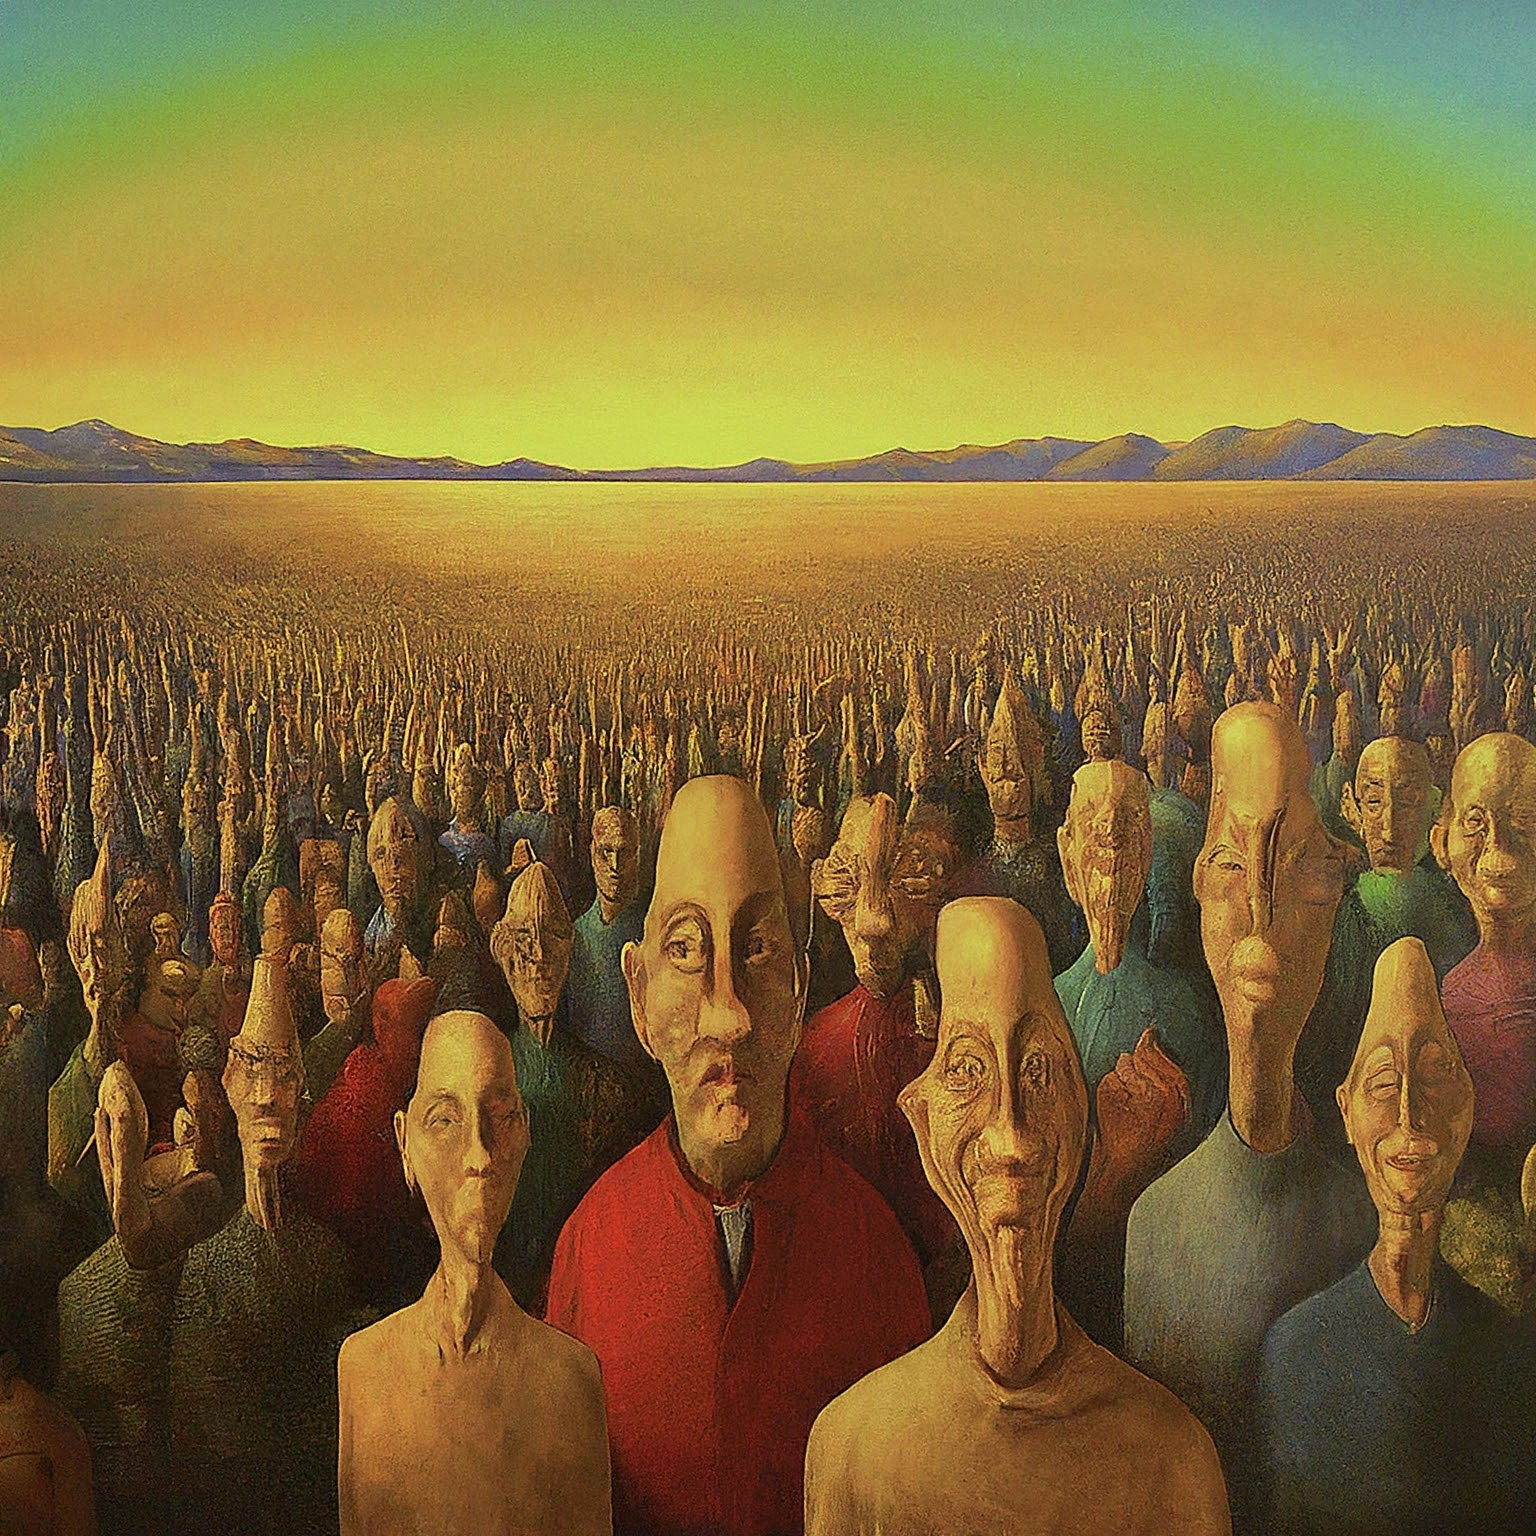
\includegraphics[height=\paperheight,width=\paperwidth]{FIGS/population-models-Gemini_Generated_Image_r55bcer55bcer55b.jpeg}
    };
    \node[anchor=north east,
    inner sep=5pt,
    opacity=0.9] at (current page.north east)
    {
        
\includegraphics[width=0.2\textwidth]{FIGS/UM-logo-horizontal-CMYK.png}
    };
    \node[anchor=south, 
    align=justify, 
    text=black, 
    text width=1.1\textwidth,
    font=\footnotesize]  (land_acknowledgement)
    at (current page.south) 
    {The University of Manitoba campuses are located on original lands of Anishinaabeg, Ininew, Anisininew, Dakota and Dene peoples, and on the National Homeland of the Red River Métis.\\
    We respect the Treaties that were made on these territories, we acknowledge the harms and mistakes of the past, and we dedicate ourselves to move forward in partnership with Indigenous communities in a spirit of Reconciliation and collaboration.};  
    \node[align=center, anchor=south,
    above=0.5cm of land_acknowledgement,
    text=black,
    font=\bfseries] {Fall 2024};
\end{tikzpicture}
  \setbeamercolor{title}{fg=subsub_header_section}
  \setbeamercolor{author}{fg=subsub_header_section} 
  \setbeamerfont{title}{size=\Large,series=\bfseries}
  \setbeamerfont{author}{size=\Large,series=\bfseries}
  \setbeamerfont{date}{series=\bfseries}
	\titlepage
\end{frame}
\addtocounter{page}{-1}


%%%%%%%%%%%%%%%%%%%%%%%%%%%%%%%%%
%%%%%%%%%%%%%%%%%%%%%%%%%%%%%%%%%
%%%%%%%%%%%%%%%%%%%%%%%%%%%%%%%%%
%%%%%%%%%%%%%%%%%%%%%%%%%%%%%%%%%
% The outline page
\begin{frame}[noframenumbering,plain]
  \begin{tikzpicture}[remember picture,overlay]
    \node[above right,inner sep=0pt,opacity=0.2] at (current page.south west)
    {
        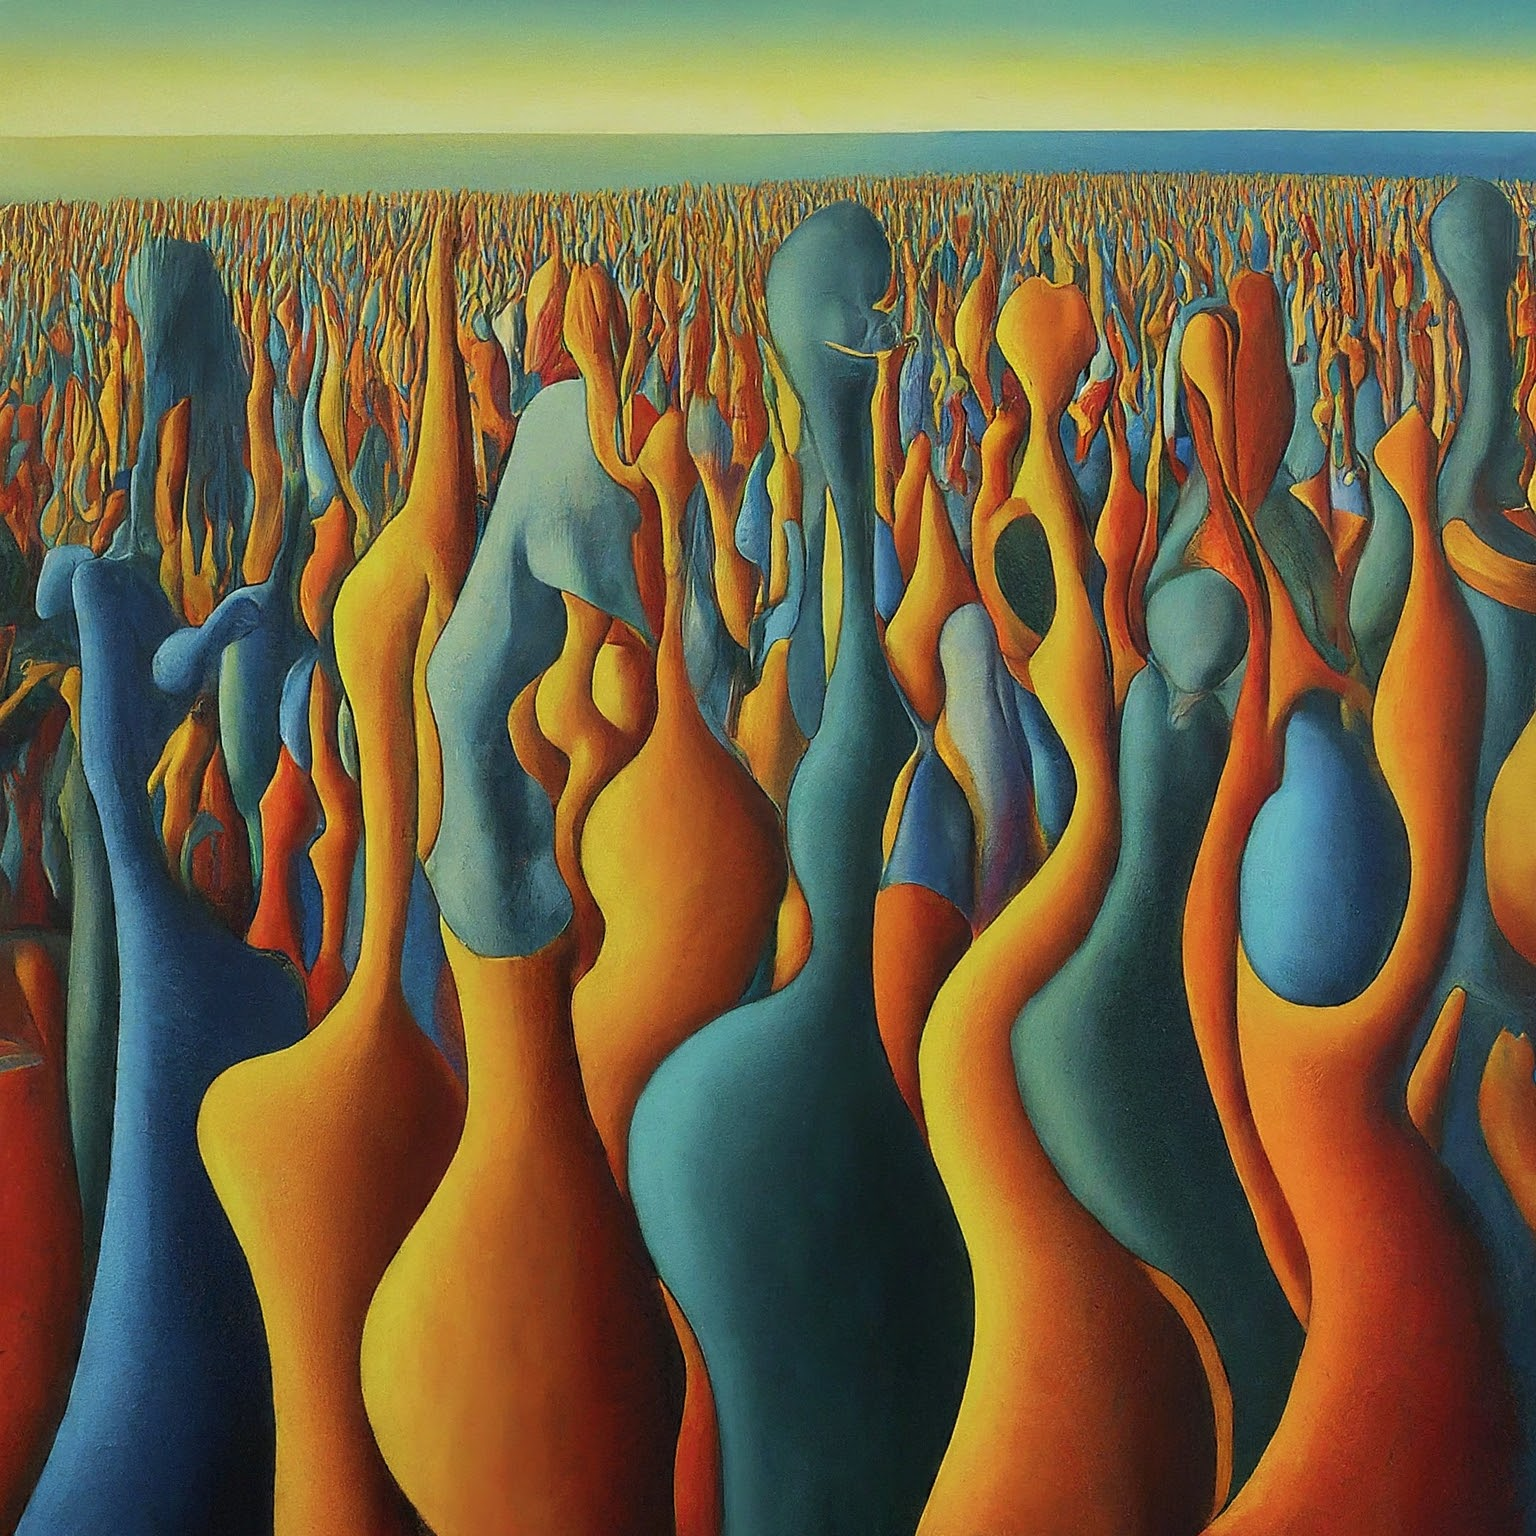
\includegraphics[height=\paperheight,width=\paperwidth]{FIGS/population-models-Gemini_Generated_Image_r55bccr55bccr55b.jpeg}
    };
  \end{tikzpicture}
  \setbeamercolor{section in toc}{fg=subsub_header_section}
  \setbeamerfont{section in toc}{size=\Large,series=\bfseries}
  \frametitle{\textcolor{blue}{\LARGE\bfseries Outline}}
  \tableofcontents[hideallsubsections]
\end{frame}
\addtocounter{page}{-1}



%%%%%%%%%%%%%%%%%%%
%%%%%%%%%%%%%%%%%%%
%%%%%%%%%%%%%%%%%%%
%%%%%%%%%%%%%%%%%%%
\section{Time spent in a state}
\frame[plain]{\tableofcontents[current]}
%\frame[plain]{\addtocounter{page}{-1}\tableofcontents[current]}


\frame{\frametitle{Some probability theory}
We suppose that a system can be in two states, $S_1$ and $S_2$.
\begin{itemize}
\item At time $t=0$, the system is in state $S_1$.
\item An event happens at some time $t=\tau$, which triggers the switch from state $S_1$ to state $S_2$.
\end{itemize}
A \textbf{random variable} is a variable that takes random values, that is, a mapping from random experiments to numbers. 

\vskip1cm
Let us call $T$ the random variable 
\begin{quote}
``time spent in state $S_1$ before switching into state $S_2$''
\end{quote}
}

\frame{
These states can be anything:
\begin{itemize}
\item $S_1$: working, $S_2$: broken;
\item $S_1$: infected, $S_2$: recovered;
\item $S_1$: alive, $S_2$: dead;
\item $\ldots$
\end{itemize}
\vskip0.5cm
We take a collection of objects or individuals that are in state $S_1$ and want some law for the \textbf{distribution} of the times spent in $S_1$, i.e., a law for $T$.
\vskip0.5cm
For example, we make light bulbs and would like to tell our customers that on average, our light bulbs last 200 years..
\vskip0.5cm
For this, we conduct an \textbf{infinite} number of experiments, and observe the time that it takes, in every experiment, to switch between $S_1$ and $S_2$.
\vskip0.5cm
From this, we deduce a model, which in this context is called a \textbf{probability distribution}.
}

\frame{
\begin{center}
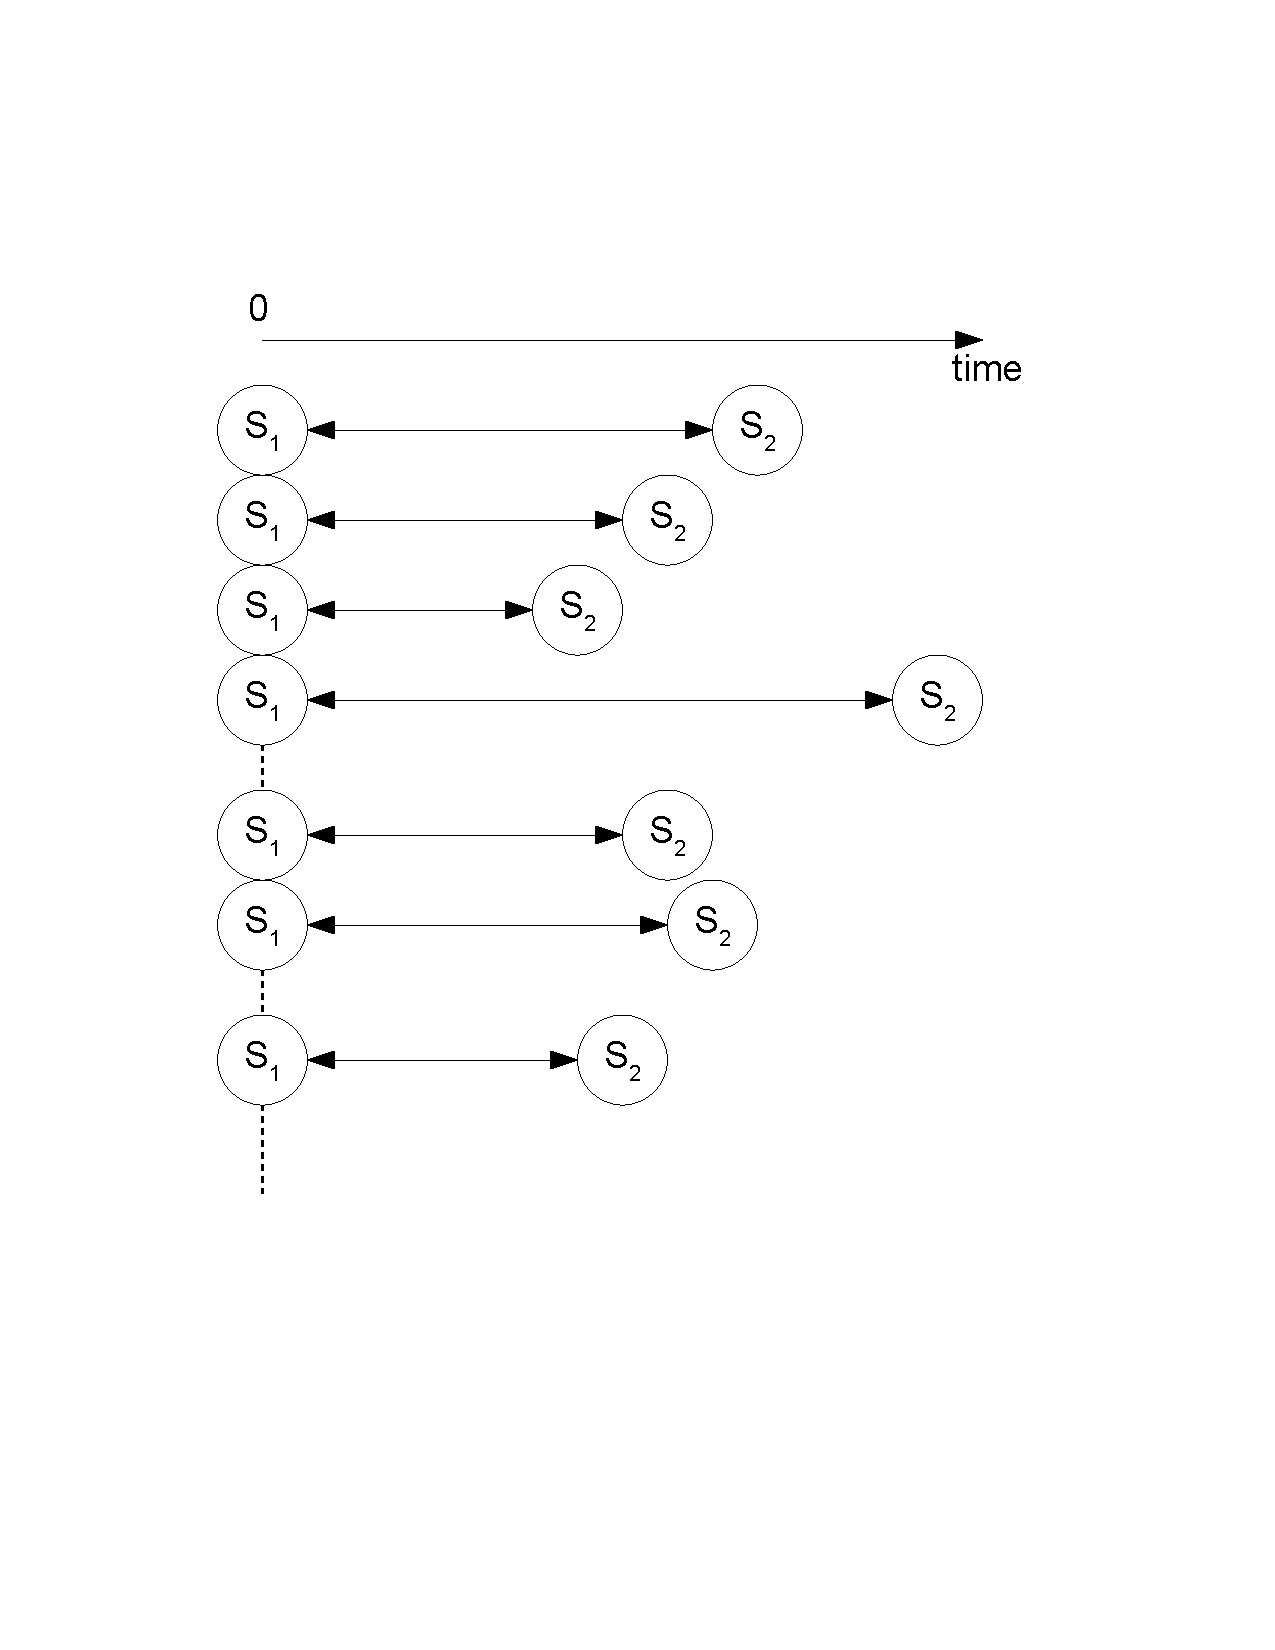
\includegraphics[height=0.95\textheight]{FIGS/random_length_sample}
\end{center}
}


\frame{\frametitle{Discrete versus continuous random variables}
We assume that $T$ is a \textbf{continuous} random variable, that is, $T$ takes continuous values. Examples of continuous r.v.: 
\begin{itemize}
\item height or age of a person (if measured very precisely)
\item distance
\item time
\end{itemize}

\vskip1cm
Another type of random variables are \textbf{discrete} random variables, which take values in a denumerable set. Examples of discrete r.v.:
\begin{itemize}
\item heads or tails on a coin toss
\item the number rolled on a dice
\item height of a person, if expressed rounded without subunits, age of a person in years (without subunits)
\end{itemize}
}

\frame{\frametitle{Probability}
A \textbf{probability} is a function $\mathcal{P}$, from a probability space to $[0,1]$.
\vskip1cm
Formally: $(\Omega,\mathcal{F},\mathcal{P})$ is a probability space, with $\Omega$ the \textbf{sample} space, $\mathcal{F}$ a $\sigma$-algebra of subsets of $\Omega$ whose elements are the \textbf{events}, and $\mathcal{P}$ a \textbf{measure} from $\mathcal{F}$ to $[0,1]$ such that $\mathcal{P}(E)\geq 0$, $\forall E\subset\Omega$, $\mathcal{P}(\Omega)=1$ and $\mathcal{P}(E_1\cup E_2\cup\cdots)=\sum_i\mathcal{P}(E_i)$.
\vskip1cm
Gives the likelihood of an event occurring, among all the events that are possible, in that particular setting. For example, $\IP{\textrm{getting heads when tossing a coin}}=1/2$ and $\IP{\textrm{getting tails when tossing a coin}}=1/2$.
}

\frame{\frametitle{Probability density function}
Since $T$ is continuous, it has a continuous \textbf{probability density function}, $f$.
\begin{itemize}
\item $f\geq 0$,
\item $\int_{-\infty}^{+\infty}f(s)ds=1$.
\item $\IP{a\leq T\leq b}=\int_a^bf(t)dt$.
\end{itemize}
\begin{center}
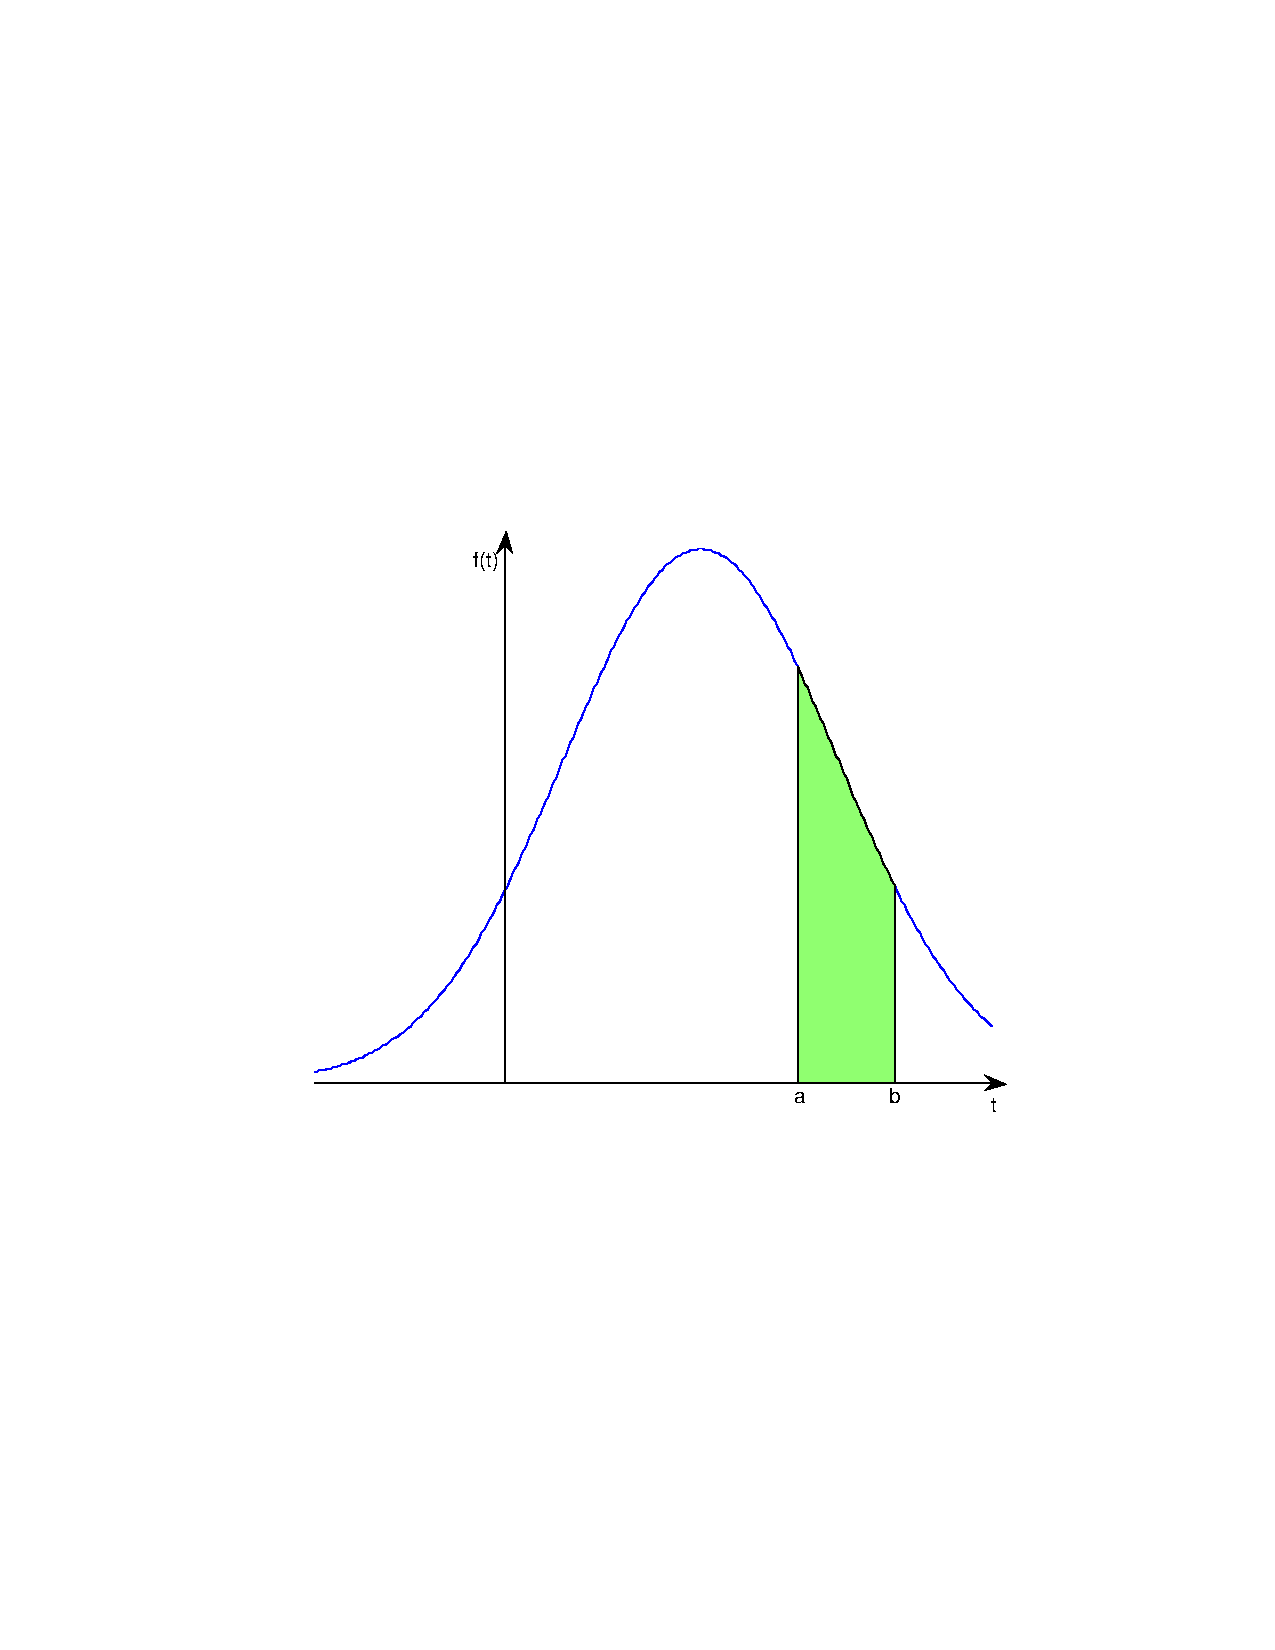
\includegraphics[width=0.6\textwidth]{FIGS/distrib_a_b}
\end{center}
}

\frame{\frametitle{Cumulative distribution function}
The cumulative distribution function (c.d.f.) is a function $F(t)$ that characterizes the distribution of $T$, and defined by
\[
F(s)=\IP{T\leq s}=\int_{-\infty}^sf(x)dx.
\]
\begin{center}
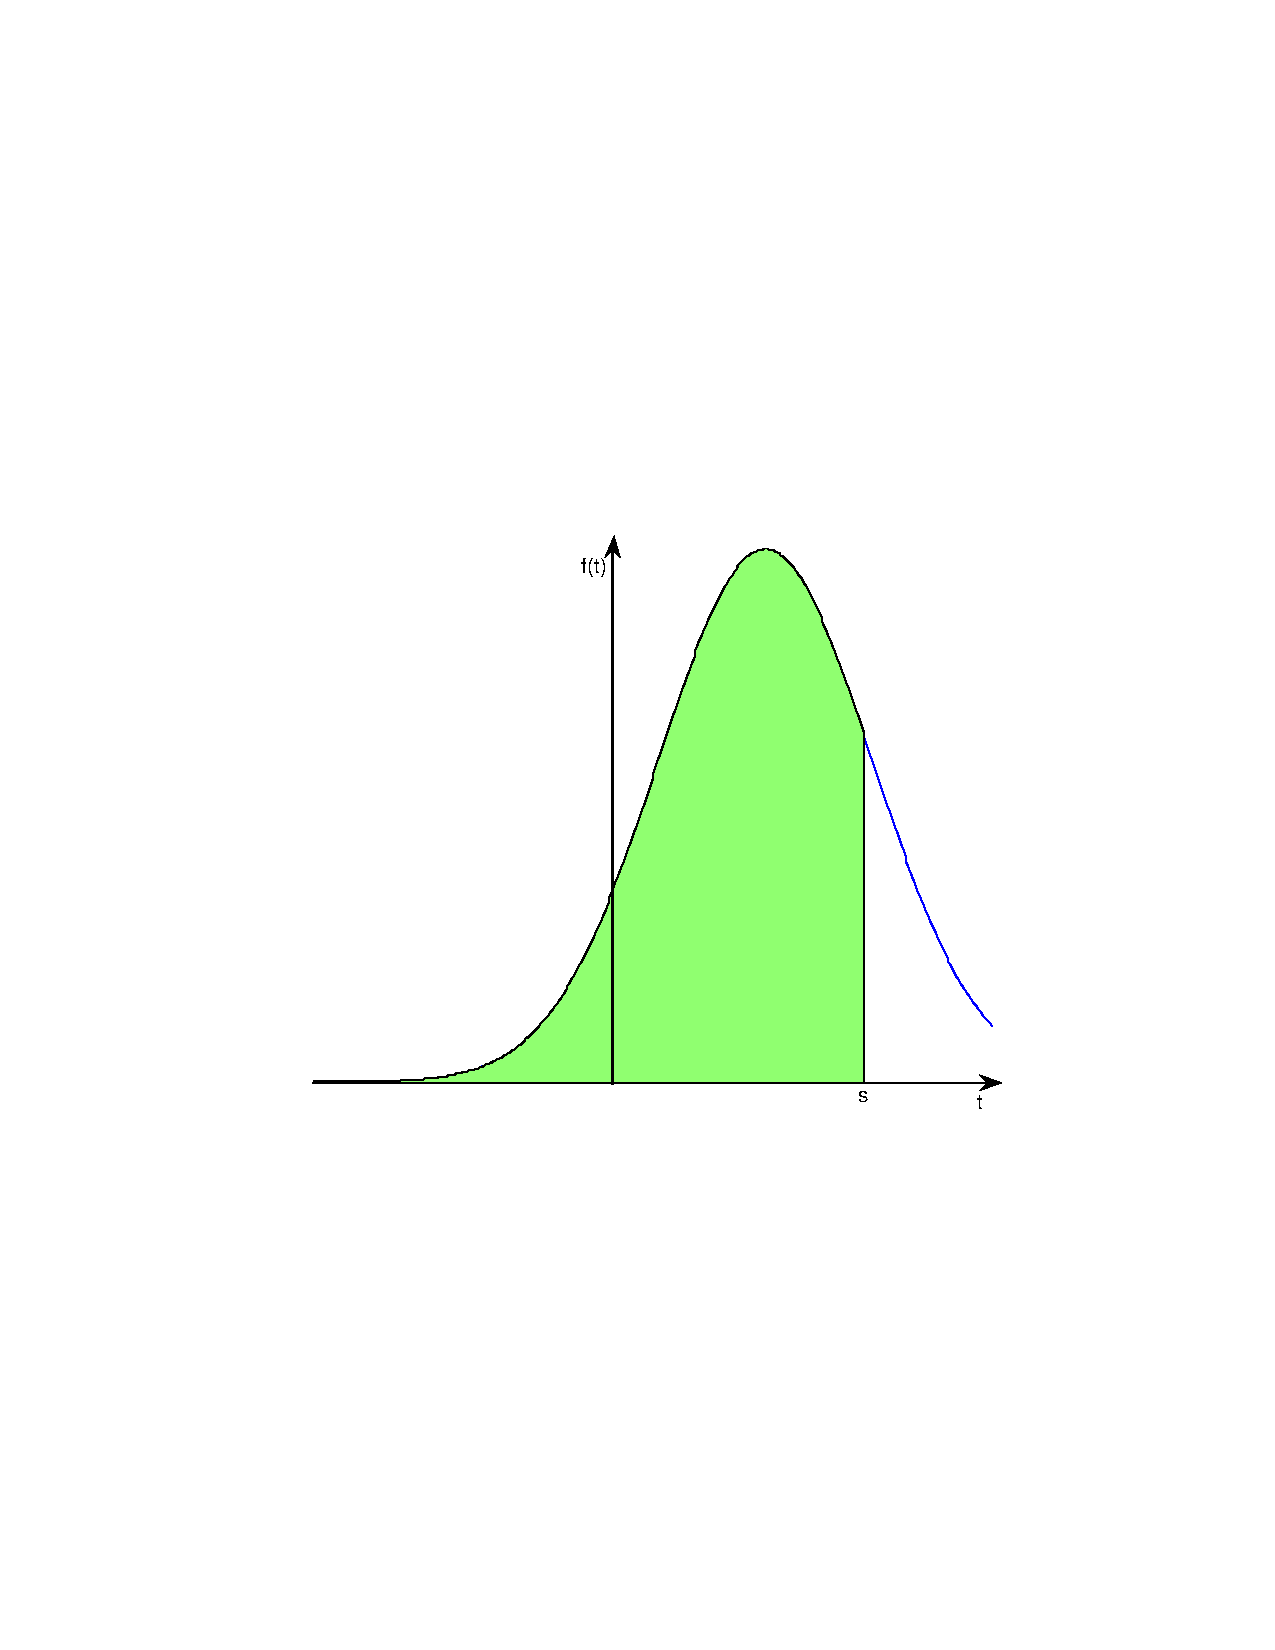
\includegraphics[width=0.6\textwidth]{FIGS/cdf_auc}
\end{center}
}

\frame{\frametitle{Properties of the c.d.f.}
\begin{itemize}
\item
Since $f$ is a nonnegative function, $F$ is nondecreasing.
\item
Since $f$ is a probability density function, $\int_{-\infty}^{+\infty}f(s)ds=1$, and thus $\lim_{t\to\infty}F(t)=1$.
\end{itemize}
\begin{center}
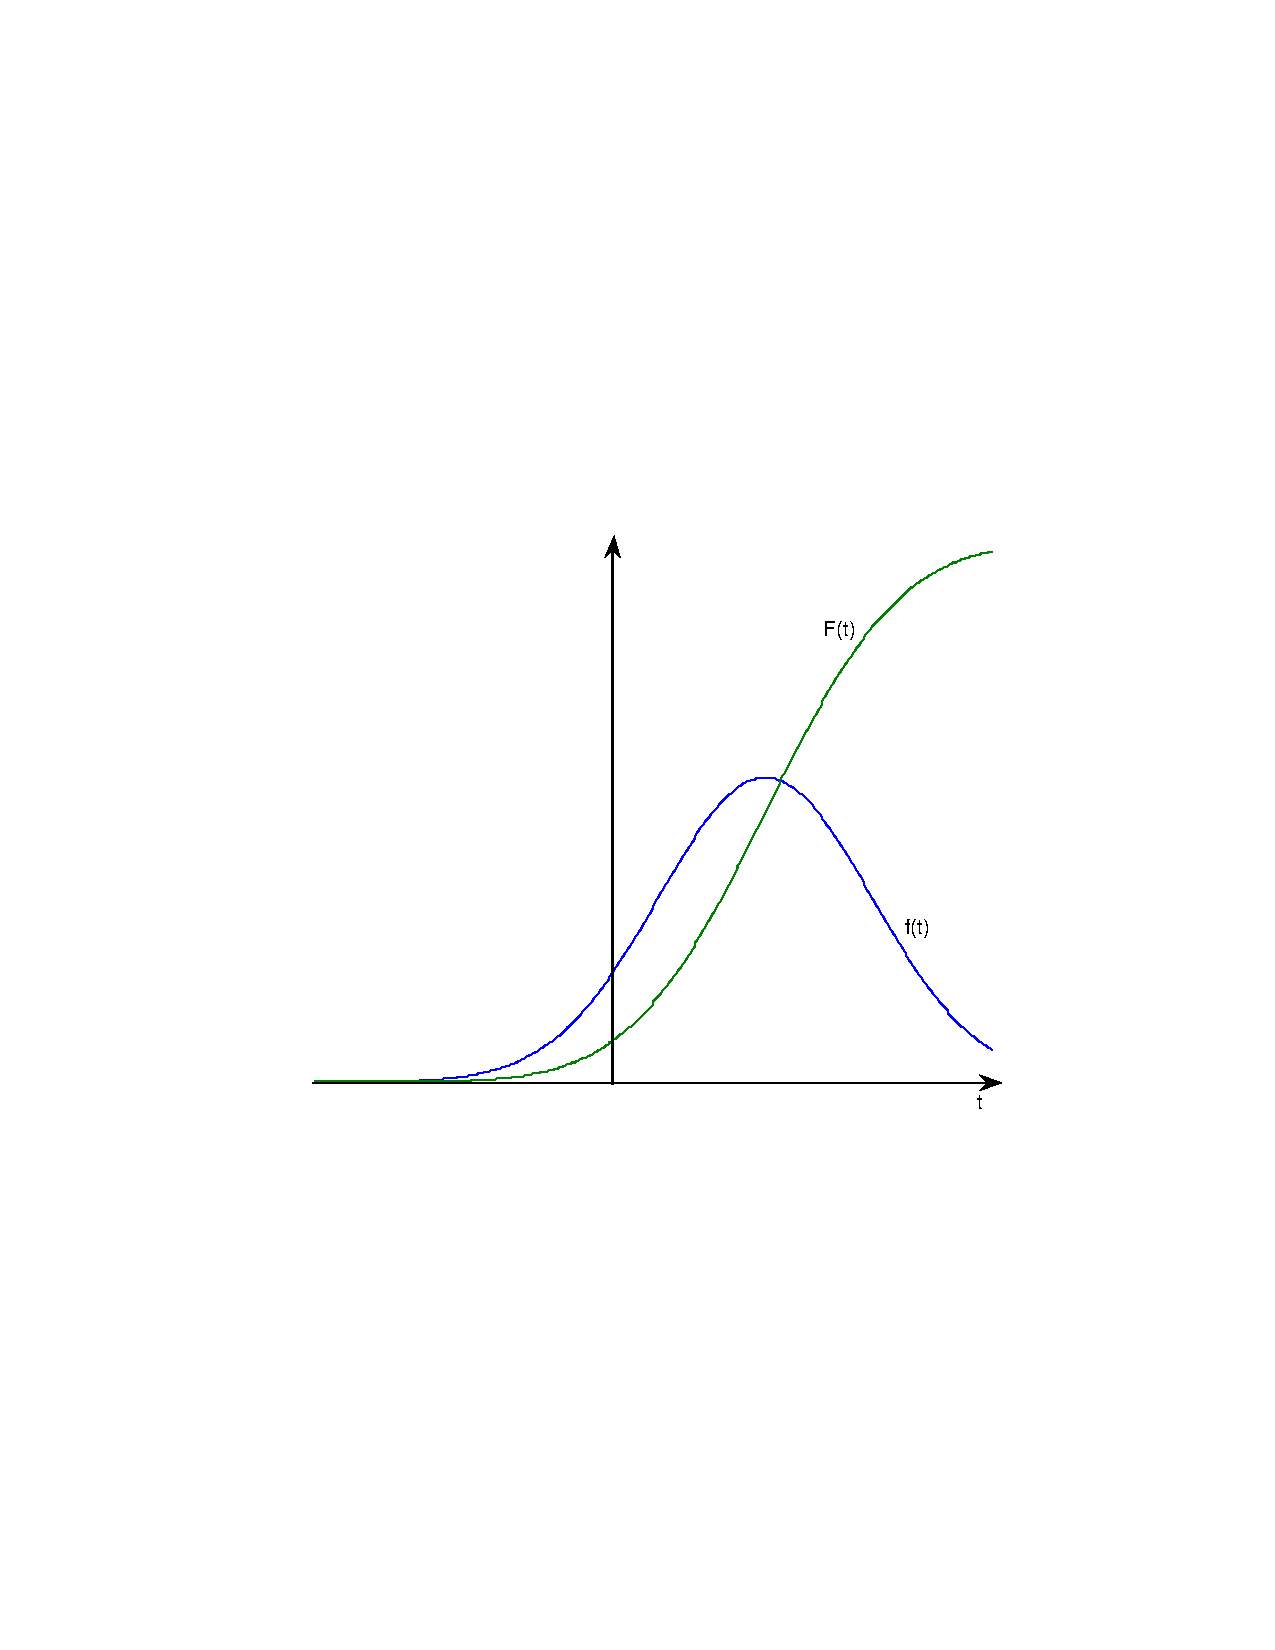
\includegraphics[width=0.6\textwidth]{FIGS/cdf_plot}
\end{center}
}

\frame{\frametitle{Mean value}
For a continuous random variable $T$ with probability density function $f$, the \textbf{mean} value of $T$, denoted $\bar T$ or $E(T)$, is given by
\[
E(T)=\int_{-\infty}^{+\infty} tf(t)dt.
\]
}


\frame{\frametitle{Survival function}
Another characterization of the distribution of the random variable
$T$ is through the \textbf{survival} (or \textbf{sojourn}) function. 

\vskip1cm
The survival function of state $S_1$ is given by 
\begin{equation}
  \S(t)=1-F(t)=\IP{T>t}
  \label{eq:survival}
\end{equation}
This gives a description of the \textbf{sojourn time} of a
system in a particular state (the time spent in the state).
\vskip1cm
$\S$ is a nonincreasing function (since $\S=1-F$
with $F$ a c.d.f.), and
$\S(0)=1$ (since $T$ is a positive random variable).
}

\frame{
The \textbf{average sojourn time} $\tau$ in state $S_1$ is given by
\[
\tau=E(T)=\int_0^\infty tf(t)dt
\]
Assuming that $\lim_{t\to\infty}t\S(t)=0$ (which is verified
for most probability distributions), 
\[
\tau=\int_0^\infty \S(t)dt
\]
}

\section{Exponential distribution}
\frame[plain]{\tableofcontents[current]}
%\frame[plain]{\addtocounter{page}{-1}\tableofcontents[current]}

\frame{\frametitle{The exponential distribution}
The random variable $T$ has an \textbf{exponential} distribution if its probability density function takes the form
\begin{equation}\label{eq:exp_distrib}
f(t)=\begin{cases}0&\textrm{if }t<0,\\
\theta e^{-\theta t}&\textrm{if }t\geq 0,
\end{cases}
\end{equation}
with $\theta>0$. Then the
survival function for state $S_1$ is of the form $\S(t)=e^{-\theta
  t}$, for $t\geq 0$, and the average sojourn time in state $S_1$ is
\[
\tau=\int_0^\infty e^{-\theta t}dt=\frac 1\theta
\]
}

\frame{
If on the other hand, for some constant $\omega>0$,
\[
\S(t)=
\left\{
\begin{array}{ll}
1, & 0\leq t\leq\omega \\
0, & \omega<t
\end{array}
\right.
\]
which means that $T$ has a Dirac delta distribution
$\delta_\omega(t)$, then the average sojourn time is a constant, namely
\[
\tau=\int_0^\omega dt=\omega
\]
These two distributions can be regarded as extremes.
}

\section{A cohort model} 
\frame[plain]{\tableofcontents[current]}

\frame{\frametitle{A model for a cohort with one cause of death}
We consider a population consisting of individuals born at the same time (a \textbf{cohort}), for example, the same year.

\vskip1cm
We suppose
\begin{itemize}
\item At time $t=0$, there are initially $N_0>0$ individuals.
\item All causes of death are compounded together. 
\item The time until death, for a given individual, is a random variable $T$, with continuous probability density distribution $f(t)$ and survival function $P(t)$.
\end{itemize}
}

\frame{\frametitle{The model}
Denote $N(t)$ the population at time $t\geq 0$. Then
\begin{equation}\label{eq:N_general}
N(t)=N_0P(t).
\end{equation}
\begin{itemize}
\item $N_0P(t)$ gives the proportion of $N_0$, the initial population, that is still alive at time $t$.
\end{itemize}
}

\frame{\frametitle{Case where $T$ is exponentially distributed}
Suppose that $T$ has an exponential distribution with mean $1/d$ (or parameter $d$), $f(t)=de^{-dt}$. Then the survival function is $P(t)=e^{-dt}$, and \eqref{eq:N_general} takes the form
\begin{equation}\label{eq:N}
N(t)=N_0e^{-dt}.
\end{equation}
Now note that
\begin{align*}
\frac{d}{dt} N(t) &= -dN_0e^{-dt} \\
&= -dN(t),
\end{align*}
with $N(0)=N_0$.
\vskip1cm
{\red $\Rightarrow$} The ODE $N'=-dN$ makes the assumption that the life expectancy at birth is exponentially distributed.
}


\frame{\frametitle{Case where $T$ has a Dirac delta distribution}
Suppose that $T$ has a Dirac delta distribution at $t=\omega$, giving the survival function 
\[
P(t)=\begin{cases}
1, & 0\leq t\leq\omega,\\
0, & t>\omega.
\end{cases}
\]
Then \eqref{eq:N_general} takes the form
\begin{equation}\label{eq:N2}
N(t)=\begin{cases}
N_0, & 0\leq t\leq\omega,\\
0, & t>\omega.
\end{cases}
\end{equation}
All individuals survive until time $\omega$, then they all die at time $\omega$.
\vskip1cm
Here, we have $N'=0$ everywhere except at $t=\omega$, where it is undefined.
}

\section{Sojourn times in an SIS disease transmission model} 
\frame[plain]{\tableofcontents[current]}

\frame{\frametitle{Models of diseases}
Consider
\begin{itemize}
\item a disease,
\item a population of individuals who can be infected by this disease.
\end{itemize}
\vskip1cm
Both can be anything:
\begin{itemize}
\item a human population subject to influenza,
\item an animal population subject to foot and mouth disease,
\item a rumor spreading in a human population,
\item inovation spreading through businesses,
\item a computer virus spreading on the internet,
\item $\ldots$
\end{itemize}
}

\frame{\frametitle{Status of individuals}
Suppose that individuals can be identified with respect to their epidemiological status:
\begin{itemize}
\item susceptible to the disease,
\item infected by the disease,
\item recovered from the disease,
\item $\ldots$
\end{itemize}
\vskip1cm
These states are clearly of the type we were discussing before.
}

\frame{\frametitle{An SIS model}
Consider a disease that confers no immunity. In this case,
individuals are either
\begin{itemize}
\item \textbf{susceptible} to the disease, with the number of such individuals at time $t$ denoted by $S(t)$,
\item or \textbf{infected} by the disease (and are also \textbf{infective} in the sense that they propagate the disease), with the number of such individuals at time $t$ denoted by $I(t)$.
\end{itemize}
\vskip1cm
We want to model the evolution with time of $S$ and $I$ ($t$ is omitted unless necessary).
\vskip1cm
{\bf\red Extremely important:} State all your hypotheses.
}

\frame{\frametitle{Hypotheses}
\begin{itemize}
\item Individuals typically recover from the disease.
\item The disease does not confer immunity.
\item There is no birth or death.
\item Infection is of \textbf{standard incidence} type
\end{itemize}
\vskip1cm
Once your hypotheses are stated, detail them if need be.
}

\frame{\frametitle{Recovery and No immunity}
Individuals recover from the disease: the infection is not permanent.
\vskip1cm
Upon recovery from the disease, an individual becomes susceptible again immediately.
\vskip1cm
Good description for diseases that confer no immunity, e.g.,
\begin{itemize}
\item the cold,
\item gonorrhea,
\item $\ldots$
\end{itemize}

}

\frame{\frametitle{No birth or death}
Suppose that
\begin{itemize}
\item the time period of interest is short,
\item the population is large enough,
\end{itemize}
then it is reasonable to assume that the total population is constant, in the absence of disease.
\vskip1cm
For mild diseases (cold, etc.), there are very little risks of dying from the disease. We assume no disease-induced death.
\vskip2cm
Hence $N\equiv N(t)=S(t)+I(t)$ is the (constant) total population.
}

\frame{\frametitle{Standard incidence}
New infectives result from random contacts between susceptible and infective individuals, described using standard incidence:
\[
\beta\frac{SI}{N},
\]
\begin{itemize}
\item $\beta SI/N$ is a rate (per unit time), 
\item $\beta$ is the \textbf{transmission coefficient}, giving probability of transmission of the disease in case of a
contact, times the number of such contacts made by an infective per
unit time.
\end{itemize}
}

\frame{\frametitle{Recovery}
We have not yet stated our hypotheses on the recovery process..

\vskip1cm
Traditional epidemiological models assume recovery from disease
with a rate constant $\gamma$.
\vskip1cm
Here, assume that, of the individuals who have become infective at time $t_0$, a
fraction $P(t-t_0)$ remain infective at time $t\geq t_0$. 
\vskip1cm
Thus, considered for $t\geq 0$, the function $P(t)$ is a survival
function.
}

\frame{\frametitle{A flow diagram for the model}
This is the \textbf{flow diagram} of our model:
\begin{center}
    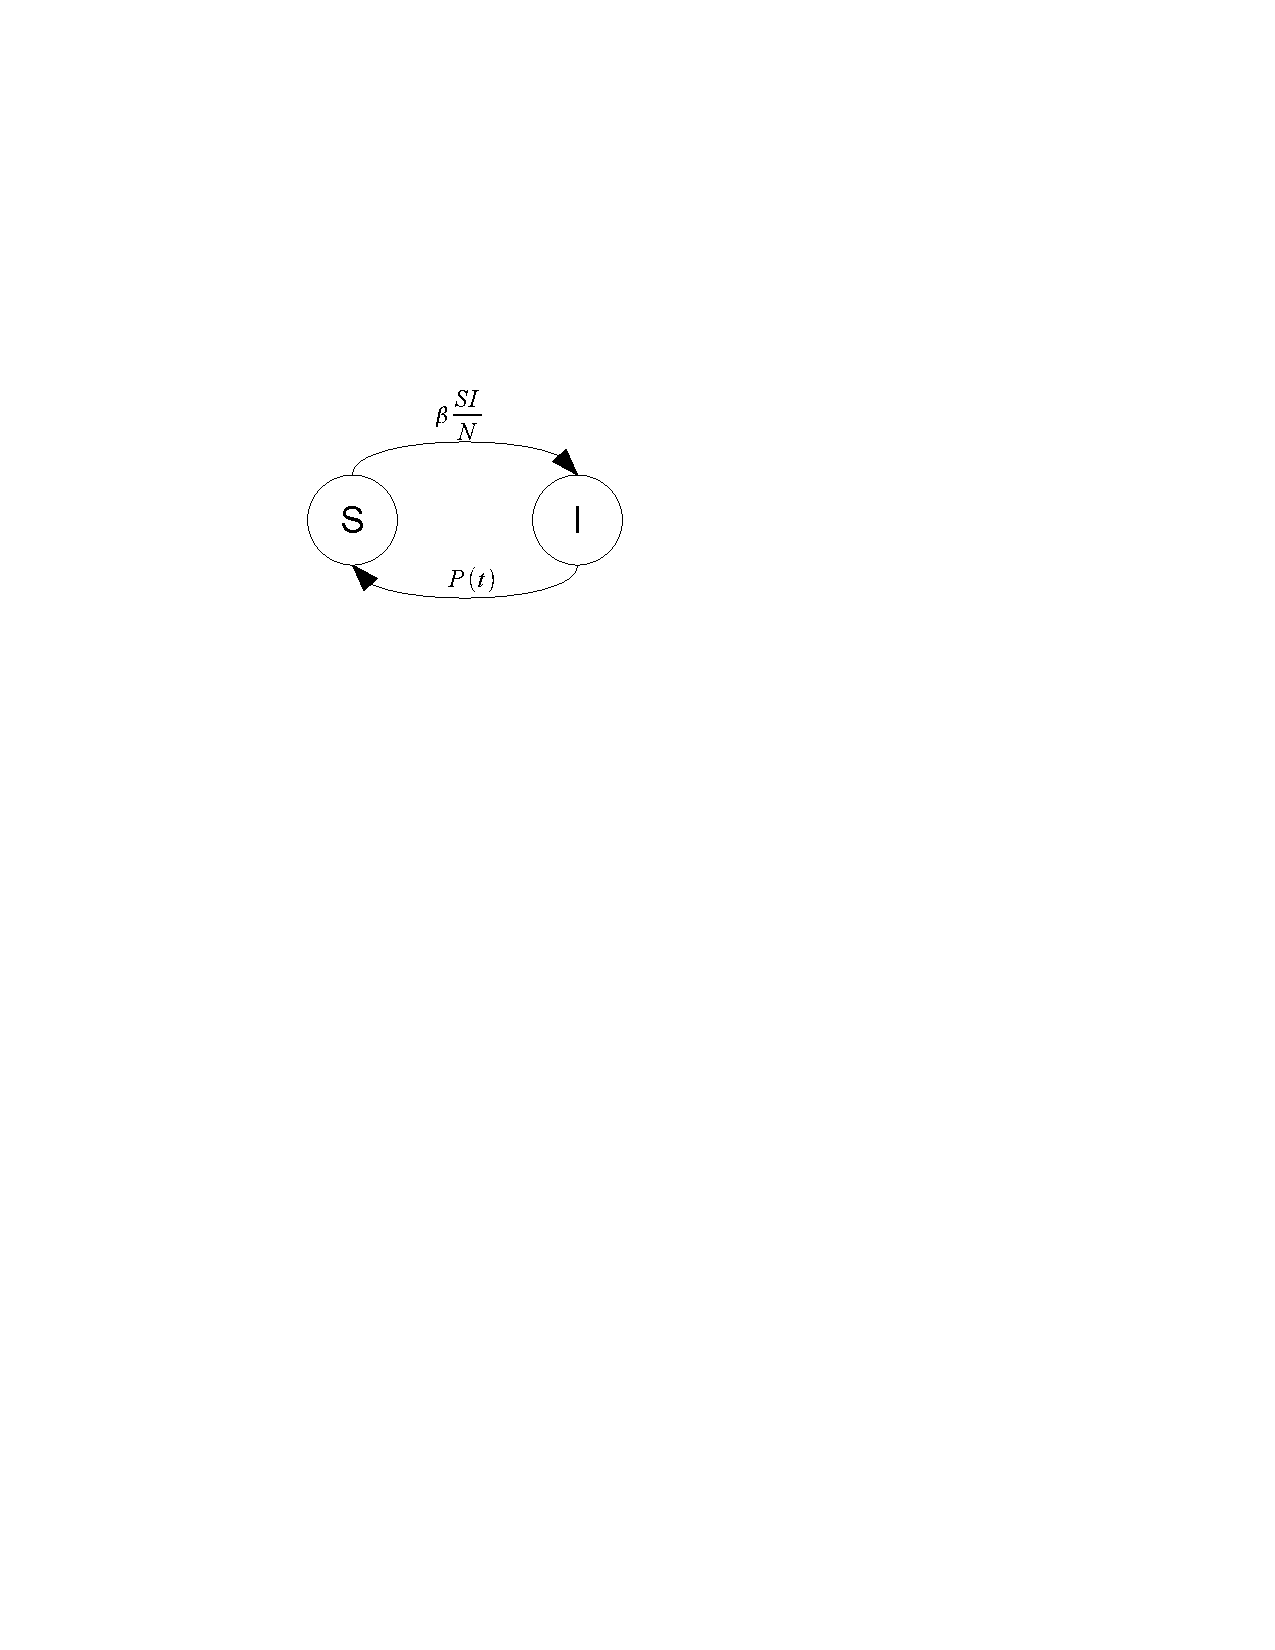
\includegraphics[width=0.5\textwidth]{FIGS/SIS_general}
\end{center}
It details the flows of individuals between the compartments in the system.

\vskip1cm
It is extremely useful to rapidly understand what processes are modelled.
}


\frame{\frametitle{Reducing the dimension of the problem}
To formulate our model, we would in principle require an equation for $S$ and an equation for $I$.

\vskip1cm
But we have
\[
S(t)+I(t)=N, \textrm{ or equivalently, }S(t)=N-I(t).
\]
$N$ is constant (equal total population at time $t=0$), so we can deduce the value of $S(t)$, once we know $I(t)$, from the equation $S(t)=N-I(t)$.

\vskip1cm
We only need to consider 1 equation. \textbf{Do this when possible!} (nonlinear systems are hard, one less equation can make a lot of difference)
}

\frame{\frametitle{Model for infectious individuals}
Integral equation for the number of infective individuals: 
\begin{equation}
I(t) = I_0(t)+ \int_0^t\beta\frac{(N-I(u))I(u)}{N} P(t-u) du
\label{eq:SIS_I} 
\end{equation}
\begin{itemize}
\item $I_0(t)$ number of individuals who were infective at time
$t=0$ and still are at time $t$.
\begin{itemize}
\item $I_0(t)$ is nonnegative, nonincreasing, and
such that $\lim_{t\to\infty}I_0(t)=0$.
\end{itemize}
\item $P(t-u)$ proportion of individuals who became infective at time $u$ and
who still are at time $t$.
\item $\beta (N-I(u))S(u)/N$ is $\beta S(u)I(u)/N$ with $S(u)=N-I(u)$, from the reduction of dimension.
\end{itemize}
}


\frame{\frametitle{Expression under the integral}
Integral equation for the number of infective individuals: 
\begin{equation}
I(t) = I_0(t)+ \int_0^t\beta\frac{(N-I(u))I(u)}{N} P(t-u) du
\tag{\ref{eq:SIS_I}} 
\end{equation}
The term
\[
\beta\frac{(N-I(u))I(u)}{N} P(t-u)
\]
\begin{itemize}
\item $\beta (N-I(u))I(u)/N$ is the rate at which new infectives are created, at time $u$,
\item multiplying by $P(t-u)$ gives the proportion of those who became infectives at time $u$ and who still are at time $t$.
\end{itemize}
Summing over $[0,t]$ gives the number of infective individuals at time $t$.
}


\frame{\frametitle{Case of an exponentially distributed time to recovery}
Suppose that $P(t)$ is such that the sojourn time in the infective
state has an exponential distribution with mean $1/\gamma$,
\emph{i.e.}, $P(t)=e^{-\gamma t}$.
\vskip0.5cm
Then the initial condition function $I_0(t)$ takes the form
\[
I_0(t)=I_0(0)e^{-\gamma t},
\]
with $I_0(0)$ the number of infective individuals at time $t=0$. This is obtained by considering the cohort of initially infectious individuals, giving a model such as \eqref{eq:N_general}.
\vskip0.5cm
Equation (\ref{eq:SIS_I}) becomes
\begin{equation}\label{eq:I_ODE}
I(t)=I_0(0)e^{-\gamma t}+\int_0^t \beta\frac{(N-I(u))I(u)}{N} e^{-\gamma (t-u)}du.
\end{equation}
}

\frame{
Taking the time derivative of \eqref{eq:I_ODE} yields
\begin{align*}
I'(t) &= -\gamma I_0(0)e^{-\gamma t}-\gamma\int_0^t \beta\frac{(N-I(u))I(u)}{N}e^{-\gamma(t-u)}du \\
&\quad +\beta \frac{(N-I(t))I(t)}{N} \\
&= -\gamma\left(I_0(0)e^{-\gamma t}+
\int_0^t \beta\frac{(N-I(u))I(u)}{N}e^{-\gamma(t-u)}du\right) \\
&\quad +\beta \frac{(N-I(t))I(t)}{N} \\
&= \beta \frac{(N-I(t))I(t)}{N}-\gamma I(t),
\end{align*}
which is the classical logistic type ordinary differential equation
(ODE) for $I$ in an SIS model without vital dynamics (no birth or death).
}

\frame{\frametitle{Case of a step function survival function}
Consider case where the time spent infected has survival function 
\[
P(t)=\begin{cases}
1, & 0\leq t\leq\omega,\\
0, & t>\omega.
\end{cases}
\]
i.e., the sojourn time in the infective state is a constant
$\omega>0$.
 
In this case (\ref{eq:SIS_I}) becomes
\begin{equation}\label{eq:I_DDE}
I(t)=I_0(t)+\int_{t-\omega}^t \beta\frac{(N-I(u))I(u)}{N} du.
\end{equation}
Here, it is more difficult to obtain an expression for $I_0(t)$. It is however assumed that $I_0(t)$ vanishes for $t>\omega$.
}

\frame{
When differentiated, \eqref{eq:I_DDE} gives, for $t\geq\omega$,
\[
I'(t)=I_0'(t)+\beta\frac{(N-I(t))I(t)}{N}
-\beta\frac{\left(N-I(t-\omega)\right)I(t-\omega)}{N}.
\]
Since $I_0(t)$ vanishes for $t>\omega$, this gives the delay
differential equation (DDE)
\[
I'(t)=\beta\frac{(N-I(t))I(t)}{N}
-\beta\frac{(N-I(t-\omega))I(t-\omega)}{N}.
\]
}

\frame{\frametitle{Conclusion}
\begin{itemize}
\item The time of sojourn in classes (compartments) plays an important role in determining the type of model that we deal with.
\item All ODE models, when they use terms of the form $\kappa X$, make the assumption that the time of sojourn in compartments is exponentially distributed.
\item At the other end of the spectrum, delay delay differential with discrete delay make the assumption of a constant sojourn time, equal for all individuals.
\end{itemize}
\vskip1cm
\begin{itemize}
\item Both can be true sometimes.. but reality is often somewhere in between.
\end{itemize}
}

\frame{
Survival function, $\S(t)=\IP{T>t}$, for an exponential distribution with mean 80 years.
\begin{center}
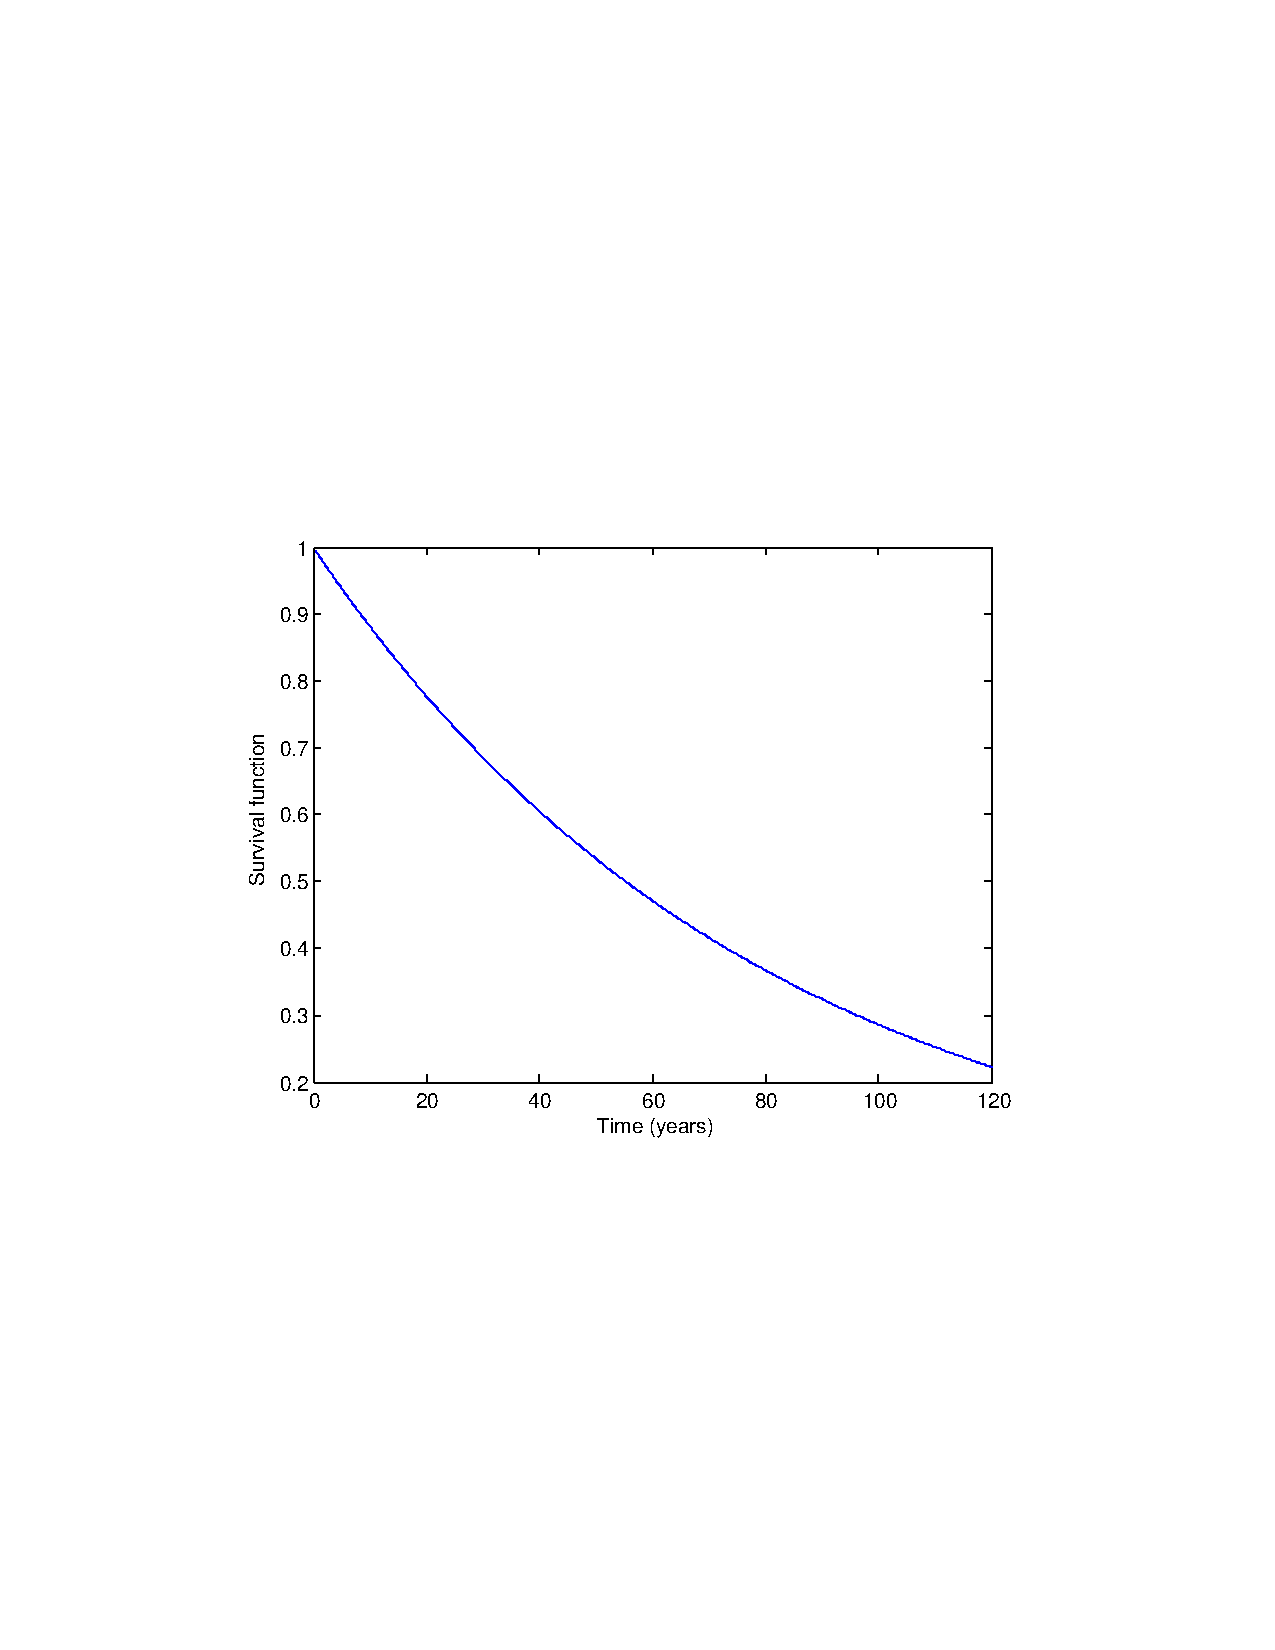
\includegraphics[width=0.7\textwidth]{FIGS/survival_exp_80years}
\end{center}
}

%\frame{
%The \textbf{basic reproduction number}, denoted by $\Rzero$, which is a
%key concept in mathematical epidemiology, is now introduced. 
%It is defined as
%the expected number of secondary cases produced, in a completely
%susceptible population, by the introduction of a typical infective
%individual.  
%For this ODE model, $\Rzero=\beta/\gamma$.
%In terms of stability, the disease free equilibrium (DFE) with $I=0$
%is stable for $\Rzero<1$ and unstable for $\Rzero>1$. 
%At the threshold $\Rzero=1$, there is a forward bifurcation
%with a stable endemic equilibrium (with $I>0$) for $\Rzero>1$. Thus
%the value of $\Rzero$ determines whether the disease dies out or tends
%to an endemic value.
%}

\end{document}
